\documentclass{article}
\usepackage{neb-macros}
\usepackage{tikz}

\begin{document}

\CheapTitle{Rings}

So far we've studied two kinds of numbers: the integers, $\ZZ$, that we know and love, and the integers modulo $n$, $\ZZ/(n)$, which are a little strange. These kinds of numbers differ in some crucial ways. For example, $\ZZ$ comes with a useful order relation $\leq$ while $\ZZ/(n)$ does not, and in $\ZZ/(n)$ it may be possible to find ``nonzero'' numbers $a$ and $b$ such that $ab \equiv_n 0$, which cannot happen in $\ZZ$. However both $\ZZ$ and $\ZZ/(n)$ have an arithmetic -- plus and times -- which behave very similarly. Addition is associative and commutative, there is a zero element, and so on.

In mathematics, when different concrete objects have behavior in common it is frequently useful to ``abstract out'' the common behavior. This is what motivates the following definition.

\begin{dfn}[Ring] \label{dfn:ring}
A \emph{ring} is a set $R$ equipped with two operations $+$ and $\cdot$, which satisfy the following properties.
\begin{itemize}
\item[A1.] $(a+b)+c = a+(b+c)$ for all $a,b,c \in R$.
\item[A2.] There is an element $0_R \in R$ (called a \emph{zero}) such that $a+0_R = 0_R+a = a$ for all $a \in R$.
\item[A3.] For every $a \in R$ there is an element $-a \in R$ (called a \emph{negative} of $a$) such that $a+(-a) = (-a)+a = 0_R$.
\item[A4.] $a + b = b + a$ for all $a,b \in R$.
\item[M.] $(ab)c = a(bc)$ for all $a,b,c \in R$.
\item[D.] $a(b+c) = ab + ac$ and $(b+c)a = ba + ca$ for all $a,b,c \in R$.
\end{itemize}
\end{dfn}

Many of the usual properties of arithmetic in $\ZZ$ can be derived as properties of any ring.

\begin{prop}
Let $R$ be a ring. Then we have the following.
\begin{enumerate}
\item The zero element of $R$ is unique in the following sense: if $a,b \in R$ such that $a+b = a$, then $b = 0_R$.
\item Negative elements in $R$ are unique in the following sense: If $a,b \in R$ such that $a+b = 0_R$, then $b = -a$.
\item $-(-a) = a$ for all $a \in R$.
\item $0_R \cdot a = a \cdot 0_R = 0_R$ for all $a \in R$.
\item $(-a)b = a(-b) = -(ab)$ for all $a,b \in R$.
\item $(-a)(-b) = ab$ for all $a,b \in R$.
\end{enumerate}
\end{prop}

\begin{proof} \mbox{}
\begin{enumerate}
\item Suppose $a+b = a$. Now $-a + (a+b) = -a + a$, and by A1 $(-a + a) + b = -a + a$. By A3 we have $0_R + b = 0_R$, and by A2 we have $b = 0_R$.
\item Suppose $a + b = 0_R$. Now $-a + (a+b) = -a + 0_R$, and by A1 we have $(-a+a)+b = -a+0_R$. By A3 we have $0_R + b = -a + 0_R$, and using A2 (twice) we have $b = -a$.
\item By definition, $(-a) + a = 0_R$, so by the uniqueness of negatives we have $a = -(-a)$.
\item Let $a \in R$. Now $a \cdot a + 0_R \cdot a = (a + 0_R) \cdot a = a \cdot a$, and so $0_R \cdot a = 0_R$. The other equality is similar.
\item Let $a,b \in R$. Now $(-a)b + ab = (-a + a)b = 0_R \cdot b = 0_R$, so that $(-a)b = -(ab)$. The other equality is similar.
\item Using the previous statement, we have \[ (-a)(-b) = -(a(-b)) = -(-(ab)) = ab. \qedhere \]
\end{enumerate}
\end{proof}

\subsection*{Examples}

\begin{itemize}
\item[$\Ints, \Ints/(n)$] The integers are a ring by definition, and we showed that the integers mod $n$ are a ring for any $n > 0$.

\item[$\QQ$] The rational numbers are a ring under the usual addition and multiplication; we will prove this later. (Actually we will define the rational numbers.)

\item[$\RR$, $\CC$] The real and complex numbers are also rings, although even defining these sets of ``numbers'' is beyond the scope of this text.

\item[$0$] The smallest possible ring must have at least one element, the zero. Suppose this is \emph{all} we have. Now the arithmetic is pretty boring: $0+0 = 0$ and $0 \cdot 0 = 0$. It is straightforward to check that these operations make the set $\{0\}$ into a ring. This example isn't very interesting, so we call this the \emph{trivial ring} or the \emph{zero ring}.

\item[$R^A$] Let $R$ be a ring, and let $A$ be any nonempty set. Then the set \[ R^A = \{ \varphi \mid \varphi : A \rightarrow R \} \] is a ring under the ``pointwise'' operations \[ (\alpha + \beta)(x) = \alpha(x) + \beta(x) \quad \mathrm{and} \quad (\alpha\beta)(x) = \alpha(x) \beta(x). \]

\item[$\MAT{2}{R}$] Let $R$ be a ring, and consider the set \[ \MAT{2}{R} = \left\{ \begin{bmatrix} a_{11} & a_{12} \\ a_{21} & a_{22} \end{bmatrix} \mid a_{11}, a_{12}, a_{21}, a_{22} \in R \right\}. \] These are just the $2 \times 2$ matrices with entries in $R$. The usual matrix addition and multiplication make $\MAT{2}{R}$ into a ring. Specifically, we define

\[\begin{bmatrix} a_{11} & a_{12} \\ a_{21} & a_{22} \end{bmatrix} + \begin{bmatrix} b_{11} & b_{12} \\ b_{21} & b_{22} \end{bmatrix} = \begin{bmatrix} a_{11} + b_{11} & a_{12} + b_{12} \\ a_{21} + b_{21} & a_{22} + b_{22} \end{bmatrix}\]

and

\[\begin{bmatrix} a_{11} & a_{12} \\ a_{21} & a_{22} \end{bmatrix} \cdot \begin{bmatrix} b_{11} & b_{12} \\ b_{21} & b_{22} \end{bmatrix} = \begin{bmatrix} a_{11}b_{11} + a_{12}b_{21} & a_{11}b_{12} + a_{12}b_{22} \\ a_{21}b_{11} + a_{22}b_{21} & a_{21}b_{12} + a_{22}b_{22} \end{bmatrix}.\]

\item[$2\Ints$] Consider the set \[ 2\Ints = \{ 2k \mid k \in \Ints \}. \] It is not too difficult to show that this set is a ring under the usual addition and multiplication of integers.

\item[$2^X$] Let $X$ be any nonempty set. The powerset $2^X$ is a ring under the operations $A + B = (A \setminus B) \cup (B \setminus A)$ and $A \cdot B = A \cap B$. This is called a \emph{ring of sets}.
\end{itemize}

\subsection*{Commutative and Unital Rings}

Our list of examples is starting to get complicated, so we make two additional definitions to start drawing distinctions among them.

\begin{dfn}
Let $R$ be a ring.
\begin{itemize}
\item We say that $R$ is \emph{commutative} if it satisfies the following property.
\begin{itemize}
\item[C.] $ab = ba$ for all $a,b \in R$.
\end{itemize}
\item We say that $R$ is \emph{unital} if it satisfies the following property.
\begin{itemize}
\item[U.] There is an element $1 \in R$ (called a \emph{one}) such that $1 \cdot a = a \cdot 1 = a$ for all $a \in R$.
\end{itemize}
\end{itemize}
\end{dfn}

\subsection*{Examples}

\begin{itemize}
\item[$\MAT{2}{R}$] If $R$ is unital, then $\MAT{2}{R}$ is also unital, with \[ 1_{\MAT{2}{R}} = \begin{bmatrix} 1_R & 0_R \\ 0_R & 1_R \end{bmatrix}. \] Is this ring ever commutative?
\end{itemize}

\begin{center}
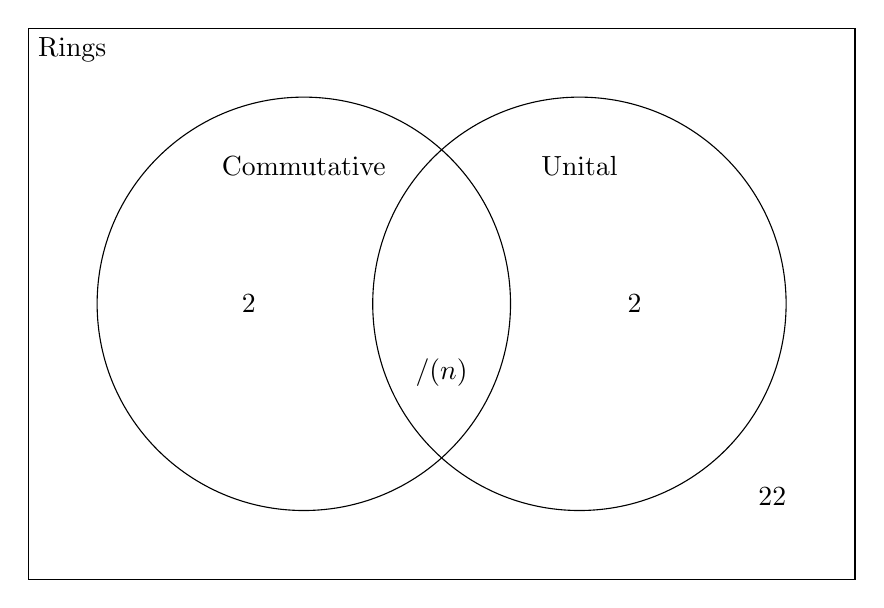
\begin{tikzpicture}[scale=0.35]
  \draw (-15,-10) -- (-15,10) -- (15,10) -- (15,-10) -- cycle;
  \draw (-5,0) circle (7.5);
  \draw (5,0) circle (7.5);
  \draw (-15,10) node [anchor=north west] {Rings};
  \draw (-5,5) node [anchor=center] {Commutative};
  \draw (5,5) node [anchor=center] {Unital};

  \draw (0,2.5) node [anchor=center] {$\ZZ$};
  \draw (0,-2.5) node [anchor=center] {$\ZZ/(n)$};
  \draw (-7,0) node [anchor=center] {$2\ZZ$};
  \draw (7,0) node [anchor=center] {$\MAT{2}{\ZZ}$};
  \draw (12,-7) node [anchor=center] {$\MAT{2}{2\ZZ}$};
\end{tikzpicture}
\end{center}

\begin{prop}
Let $R$ be a unital ring.
\begin{enumerate}
\item The one element of $R$ is unique in the following sense: if $u \in R$ such that $u \cdot a = a$ for all $a \in R$, then $u = 1$.
\item $-a = (-1) \cdot a$ for all $a \in R$.
\end{enumerate}
\end{prop}

\begin{proof} \mbox{}
\begin{enumerate}
\item Suppose $u$ is such an element. In particular, $1 = u \cdot 1 = u$.
\item Let $a \in R$. Then $a + (-1)a = 1a + (-1)a = (1 + (-1))a = 0a = 0$, so that $(-1)a = -a$. \qedhere
\end{enumerate}
\end{proof}

\subsection*{Exercises}

\begin{enumerate}
\item Let $R$ be a ring. Show that $\MAT{2}{R}$ is a ring by verifying that each of the properties in Definition \ref{dfn:ring} hold. This will be tedious.

\item Let $X$ be a nonempty set. Show that the ring of sets $2^X$ is a ring by verifying that each of the properties in Definition \ref{dfn:ring} hold. This will be tedious.

\item Let $R$ be a ring. Show that the ring $\MAT{2}{R}$ is unital if and only if $R$ is unital.

\item \textbf{Sigma Notation.} Let $R$ be a ring and $a \leq b$ integers. If $\{ r_i \mid a \leq i \leq b \}$ is a finite subset of $R$ indexed by the integers from $a$ to $b$, we define \[ \sum_{i=a}^b r_i = r_a + r_{a+1} + \cdots + r_{b-1} + r_b. \] Show that the following hold.
\begin{enumerate}
\item $\left( \sum_{i=a}^b r_i \right) + \left( \sum_{i=b}^c r_i \right) = \sum_{i=a}^c r_i$ whenever $a \leq b \leq c$.
\item $s \cdot \left( \sum_{i=a}^b r_i \right) = \sum_{i=a}^b sr_i$ and $\left( \sum_{i=a}^b r_i \right) \cdot s = \sum_{i=a}^b r_i s$.
\end{enumerate}

\item A ring $R$ is called \emph{boolean} if for all $a \in R$, we have $aa = a$. Let $R$ be a boolean ring.
\begin{enumerate}
\item Show that the ring of sets $2^X$ is boolean for any nonempy $X$.
\item Show that $-a = a$ for all $a \in R$. (Hint: consider $a+a$.)
\item Show that $R$ is commutative. (Hint: let $a,b \in R$ and consider $a+b$.)
\end{enumerate}

\item Find all the matrices $A \in \MAT{2}{\ZZ/(5)}$ such that $A^2 = 0$. This will be tedious.
\end{enumerate}

\end{document}
